% Chapter Template

\chapter{Problem Solution} % Main chapter title

\label{Chapter6} % Change X to a consecutive number; for referencing this chapter elsewhere, use \ref{ChapterX}

\lhead{Chapter 6. \emph{Problem Solution}} % Change X to a consecutive
% number; this is for the header on each page - perhaps a shortened title

%----------------------------------------------------------------------------------------
%	SECTION 1
%----------------------------------------------------------------------------------------

\section{Integrate Henshin with DPF}

DPF is a a framework where it is possible to create an arbitrary levels of
meta-models, and that gives the users the freedom to define a well formed domain
specific modeling language with support for creating an unlimited number of
meta-models and to define constraints for each specification at each level. The
framework provides the possibility to define specifications that specify
underlying specifications. Where each specification
$\spec{S}$\textsubscript{n+1} defines the abstract syntax for a specification
$\spec{S}$\textsubscript{n}. For DPF to be a framework that follows the visions
of model driven engineering it needs to have support for automation of
specifications over different levels of abstraction. It already has support for
some cases of model transformations. There is one natural model transformation
for DPF when specifying a new specification. A new specification will always
be specified by a modeling language that corresponds to a specification
$\spec{S}$\textsubscript{n+1}. These specification may either be a user created
specification or the default specification provided by the framework, that
conforms to it self. The creation of a new specification can be viewed as the
first support for automation over levels of abstraction for models that the
Diagram Predicate Framework provides. In 2012 Anders Sandven published his
master thesis\cite{Sandven_thesis}, where he implemented support for generating
source code with the DPF Editor. DPF does not provide support for applying an
exogenous model transformation to a specification described in one domain
specific modeling language to a model expressed in another domain specific
modeling language. To achieve this we want to integrate Henshin transformation
language\cite{Arendt2010} to the framework.  

\begin{figure}[H]
	\centering
	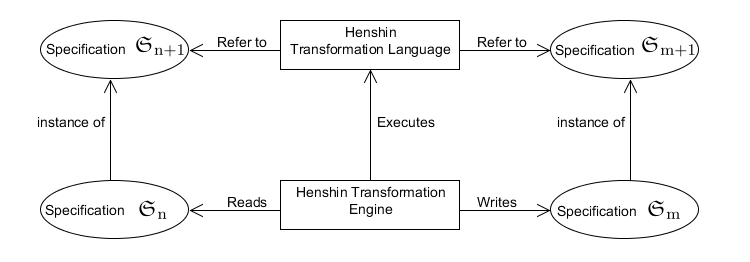
\includegraphics[scale=0.7]{./Figures/TransformationSolutionBasic.png}
	\caption[Integrating Henshin with DPF]
	{Using Henshin transformation language to translate a specification
	$\spec{S}$\textsubscript{n}.}
	\label{fig:Simple_Solution}
\end{figure}

Figure~\ref{fig:Simple_Solution} explains how we want to integrate the Henshin
transformation language, that consist of a transformation language and a
transformation engine, with DPF. We use the Henshin transformation engine to
read an instance specification $\spec{S}$\textsubscript{n} and write an instance
specification $\spec{S}$\textsubscript{m}. To achieve this the transformation
engine executes a set of transformation rules written in the Henshin
Transformation Language. These transformation rules refers to both the
specification $\spec{S}$\textsubscript{n+1} and specification
$\spec{S}$\textsubscript{m+1} that the source and target model are typed over.

The problem with integrating Henshin with DPF is that Henshin is implemented by
EMF, and therefore utilize OMG's MOF. The Henshin model transformation
language use models, that are created accordingly to the four layer
meta-modeling that MOF provides, to create the transformation rules. The
specification implementation for a DPF model is created as an EMF meta-model 
and utilize the EMF Genmodel to provide code generation. In DPF we can create an
arbitrary level of meta-models and therefore each domain specific modeling
language created in the framework can have different layers of specification
models. The Henshin environment has strict guidelines on how models are imported
and used. These models are required to be created accordingly to and typed by
the Ecore model provided by EMF. Henshin can then utilize these models to create
nodes and edges that form both the LHS and the RHS of a transformation rule. 

\begin{figure}[H]
	\centering
	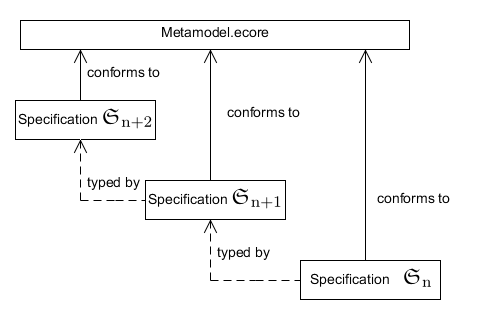
\includegraphics[scale=0.7]{./Figures/metamodelSpecification.png}
	\caption[Specification relationship with core meta-model]
	{Relationship between layers of specification.}
	\label{fig:core_metamodel}
\end{figure}

Figure~\ref{fig:core_metamodel} gives a representation on how specification
are related to one another and every specification conforms to one common
meta-model. For Henshin we can import the specification meta-model,
\textit{Meatmodel.ecore} provided by DPF. A specification
$\spec{S}$\textsubscript{1\ldots n} conforms to this meta-model regardless of
what layer it is part of. We can use this meta-model in Henshin to define the
content of the transformation rules since every specification
$\spec{S}$\textsubscript{n} conforms to this meta-model. However, other than
consisting of an underlying graph and a set of constraints, a DPF specification
$\spec{S}$\textsubscript{n} is also typed by another
specification$\spec{S}$\textsubscript{n+1}, and this is where it gets
challenging. A specification $\spec{S}$\textsubscript{n} created in the
framework is typed by a specification $\spec{S}$\textsubscript{n+1} and both
models conforms to one common meta-model, but a specification model
$\spec{S}$\textsubscript{n} is at the same time created as an instance from a
specification model $\spec{S}$\textsubscript{n+1}. This is where we have to
find a work around for our solution, because we cannot import an instance model
of an Ecore based meta-model into the Henshin model transformation environment.
The Henshin model transformation language can apply a set of transformation
rules to these instance models and execute an in-place model transformation
that change these instance models. But the transformation language can only
import and utilize models based on the Ecore meta-model. To solve this for DPF
models we expand transformation rules in Henshin with application conditions.
We will look more closely to how this is done later in this chapter, but what
we basically do is that we restrict the LHS graph to locate matching modeling
elements in an instance model based these modeling elements types.

%----------------------------------------------------------------------------------------
%	SECTION 2
%----------------------------------------------------------------------------------------

\section{Henshin meta-model}

The Henshin transformation language provides a meta-model that is an EMF based
model and uses the Ecore meta-model for typing purposes\cite{Arendt2010}. Since
this model is created based on EMF we know that EMF will generate interfaces and
a factory that we can utilize to implement Henshin transformation rules in Java.
We form a pattern graph and a replacement graph for a transformation rule based
on this Henshin factory. In the following we will address what elements a
transformation rule in Henshin consist of based on the Henshin meta-model for a
transformation rule represented in figure~\ref{fig:Henshin_metamodel}.
 

\begin{figure}[H]
	\centering
	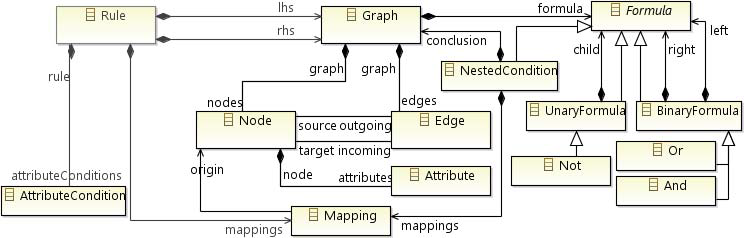
\includegraphics[scale=0.8]{./Figures/Henshin_metamodel.png}
	\caption[Henshin transformation meta-model]
	{Henshin transformation meta-model\cite{Arendt2010}.}
	\label{fig:Henshin_metamodel}
\end{figure}

A \textbf{Rule} in Henshin represents a new transformation rule that has a name,
a description and three properties. The first property disables or enables the
transformation rule, while the two other properties lets the user enable or
disable injective matching and the check dangling condition. The rule class
works as the root for all other elements present in
figure~\ref{fig:Henshin_metamodel}. A new rule defines a left hand side and a
right hand side \textbf{Graph}. The content of the LHS graph represents the
model pattern used to locate matches in an instance graph while the RHS
represents the model pattern that replaces the LHS. The lhs and rhs graph is
formed by creating nodes and edges. Nodes refers to objects in an instance graph
and edges refer to references between objects. An edge has a source and a target
node, while a node can have a collection of incoming and outgoing edges. The
nodes can also have a set of attributes attached. Nodes, edges and attributes
all have one common property, and that is that they all have a type. This type
is a reference to either an EClass, EReference or EAttribute, that is all
classes of the Ecore meta-model. For example a node that is typed by a specific
EClass will only be matched to objects of this type in an instance graph. These
nodes and edges are represented under a graph and form a pattern. Together with
the LHS and the RHS these patterns is either used to find matching patterns in
a source model or to create the corresponding pattern for a target model. A
\textbf{Mapping} is how Henshin specifies if nodes are part of both the pattern
graph and the replacement graph. This means that these objects should be part of
the matching pattern, but should not be deleted. A mapping has two properties,
namely an origin and an image. The origin property refers to a given node, while
the image property specify that another node has a mapping to this node. So far
we have a rule that can have two graphs and a set of mappings. Furthermore a
rule can also have a set of attribute conditions. 

A rule can also have application conditions that determines where a specific
rule could be applied. These application conditions are defined in the
\textbf{Formula} class and is a child of a graph. This formula can either be an
u-nary logical, a binary logical operation or a nested condition. The first
logical operation operated on a single operand while the second operates on two
operands, where these operands are represented as a conditional statement that
is either true or false. A rule can be applied to a instance graph if and only
if all application conditions are valid. We can basically have a unlimited
nested formulas in Henshin, since a binary formula can have a right and left
\textbf{Formula}, that can again be of type binary formula. Henshin however is
only concerned with if this formula is valid or invalid when a transformation
rule is applied. A nested condition is required if we want to have nodes that
are part of the LHS graphs. A nested condition provides a graph and a set of
mappings to elements that are part of the LHS graph. This graph that is child of
a nested condition contains nodes, edges and attributes that form a structural
pattern that specifies an application condition. We can observe that a
transformation rules can have several number of application conditions. A
binary formula can be of type \textbf{Or} or \textbf{And}. If the structure of a
binary formula is the latter, then all the application conditions from both the
right and left formula has to be be valid for a transformation rule to be
applied to a instance graph. 

\section{Transform Model Editor}

With the Eclipse Modeling Framework we created an Eclipse plugin where users can
create and modify transformation rules. Figure~\ref{fig:transform_metamodel}
provides the structural data model that we use to generate code for the
implementation of the model and the plugin. The two classes Transform and
Production are the two domain classes that together defines this domain specific
modeling language that lets users create transformation rules. The Transform
class represent the Transform Model Editor. It has a source meta-model and a
target meta-model, that corresponds to a source specification and a target
specification. If these two models are the same model, then the model
transformation is an endogenous model transformation or if the models are
different we have an exogenous model transformation. We also have the file
location on the storage unit for the source and target meta-model. The rules
represents a collection of the transformation rules. These rules are typed by a
Production and represent one single transformation rule. A transformation
rule has a name and contains a graph that is stored internally for each rule.
This graph contains a pattern of nodes and arrows that the user can edit to
form a LHS graph and a RHS graph. A single Production also has several
collections that contains nodes and arrows. The user can edit the internal graph
for a rule by adding nodes and arrows to one of these lists. A node and arrow
must be uniquely mapped to one of these collection of nodes and arrows. 

\begin{figure}[H]
	\centering
	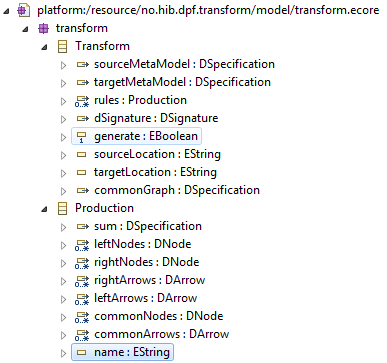
\includegraphics[scale=0.8]{./Figures/transform_metamodel.png}
	\caption[Model for the DPF transformation editor]
	{The domain model to create a DPF model transformation editor.}
	\label{fig:transform_metamodel}
\end{figure}

The user has to invoke the file creation wizard for the Transform Model Editor.
Other than choosing a project folder and a name for this new editor file, the
user has to specify what model is the source meta-model and what model is the
target meta-model. If the user do not specify a target meta-model then the file
creation wizard will interpret this as an endogenous model transformation.

The Transform Model Editor plugin has two editors that users can interact with.
The first is the master editor for the plugin and contains a list of the
transformation rules, where users can create, read, update and delete rules. The
second editor is administrated by the master editor, and each time a new
transformation rule is chosen, a simple version of the DPF editor is opened
with its corresponding transformation rule. This editor is created from the 
Graphical Editing Framework (GEF) and is a graphical editor that includes a
palette. This palette is the same palette that is used in the DPF Editor and
contains modeling elements from the source meta-model and the target meta-model.

\begin{figure}[H]
	\centering
	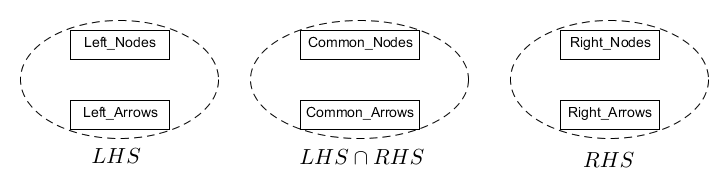
\includegraphics[scale=0.7]{./Figures/left_common_right.png}
	\caption[The three subgraphs for a transformation rule.]
	{Three subgraphs for each transformation rule in the editor.}
	\label{fig:lists_editor}
\end{figure}

These nodes and arrows are used to create the internal graph for each
corresponding rule. For each rule the users can uniquely map nodes and arrows to
three subgraphs represented as lists. Figure~\ref{fig:lists_editor} represents
the left, right and common subgraphs, where each corresponding subgraph
has a list of nodes and arrows. Each subgraph represents a different part of a
transformation rule according to graph transformation. The left subgraph
represents the LHS graph of a rule, while the right subgraph represents the RHS
graph. The common subgraph represents the intersection between the pattern
graph and the replacement graph. It is vital for the model transformation to
work that all the nodes and arrows are mapped to one of these three graphs.
This is entirely up to the user, because the nodes and arrows from the LHS
graph have to be created in such a way that the graph can be matched in an
instance graph.

Now that a list of transformation rules has been specified the user has to
generate a correspondence graph and generate transformation rules for the
Henshin model transformation language. 

\begin{enumerate}

\item Generate Correspondence Graph.

\item Generate Henshin Rules.

\item Apply Model Transformation. 

\end{enumerate}


\section{Generate Correspondence Graph}

\section{Generate Henshin Rules}

We utilize the meta-model represented in figure~\ref{fig:Henshin_metamodel} to
create transformation rules in Henshin.  We use the factory that is provided by
EMF for Henshin model transformations to create transformation rules in Henshin.
We start with creating the root element that is required for a Henshin model
transformation and import EPackages that is needed to define the content of a
transformation rule. We need to import two models if we want to translate a
specification with Henshin. The first model is the corresponding meta-model for
all specifications and the second model is the meta-model for including
traceable links in Henshin. The transformation language requires models that
define the abstract syntax for an instance model to be able to specify modeling
elements for both the LHS and the RHS of a transformation rule. We can use
the typing provided by these two models when defining new nodes, edges or
attributes in Henshin. These types will be EClass for nodes, EReference for
edges and EAttribute for attributes. Typing for nodes, edges and attributes in
Henshin are required to be able to find matches in a source model. 

For Henshin we create one rule for each production provided by the editor, where
the name of a rule is acquired from a production. For each rule Henshin provides
a LHS, a RHS graph and a collection of mappings. Now we have to create the
pattern that Henshin use to search for matches and replace these matches with a
resulting pattern. Modeling elements that form a pattern in the LHS are used to
find a match in a source model, while modeling elements that form a pattern in
the RHS are used to replace these elements. Henshin also include an intersection
graph for each rule. This graph is not represented as a graph like the LHS and
the RHS are, but is represented by having elements in both the LHS and the RHS
graph with mappings that distinguish that these elements are one and the same.
Now we have the LHS graph, the RHS graph and the intersection of these two
graphs, that we talked about in section~\ref{sec:graph_based}. 

\begin{figure}[H] 
	\centering
	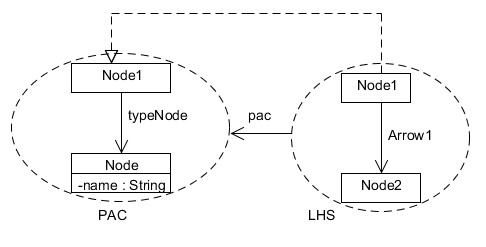
\includegraphics[scale=0.7]{./Figures/PAC_Henshin_node.png}
	\caption[How to handle node types for a rule]
	{How to find matches for types in a transformation rule.}
	\label{fig:pac_henshin}
\end{figure}

\section{Apply Model Transformation}



\begin{figure}[H]
	\centering
	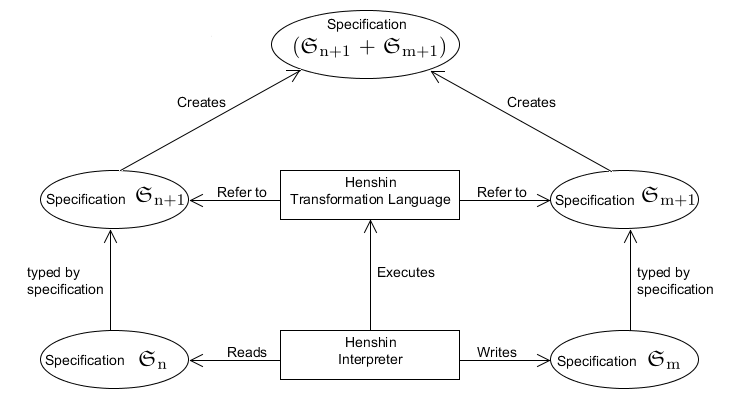
\includegraphics[scale=0.7]{./Figures/TransformationSolution_Correspond.png}
	\caption[Specification for the correspondence objects]
	{The solution expanded with a specification for the correspondence objects.}
	\label{fig:Solution_CorrespondanceObjects}
\end{figure}




\section{Integrateing Henshin with DPF Model Transformation Editor}

\section{Henhsin Editor}



